%%%%%%%%%%%%%%%%%%%%%%%%%%%%%%%%%%%%%%%%%
% Jacobs Landscape Poster
% LaTeX Template
% Version 1.0 (29/03/13)
%
% Created by:
% Computational Physics and Biophysics Group, Jacobs University
% https://teamwork.jacobs-university.de:8443/confluence/display/CoPandBiG/LaTeX+Poster
% 
% Further modified by:
% Nathaniel Johnston (nathaniel@njohnston.ca)
%
% This template has been downloaded from:
% http://www.LaTeXTemplates.com
%
% License:
% CC BY-NC-SA 3.0 (http://creativecommons.org/licenses/by-nc-sa/3.0/)
%
%%%%%%%%%%%%%%%%%%%%%%%%%%%%%%%%%%%%%%%%%

%----------------------------------------------------------------------------------------
%	PACKAGES AND OTHER DOCUMENT CONFIGURATIONS
%----------------------------------------------------------------------------------------

\documentclass[final]{beamer}

\usepackage[scale=1.24]{beamerposter} % Use the beamerposter package for laying out the poster


\usetheme{confposter} % Use the confposter theme supplied with this template

\setbeamercolor{block title}{fg=ngreen,bg=white} % Colors of the block titles
\setbeamercolor{block body}{fg=black,bg=white} % Colors of the body of blocks
\setbeamercolor{block alerted title}{fg=white,bg=dblue!70} % Colors of the highlighted block titles
\setbeamercolor{block alerted body}{fg=black,bg=dblue!10} % Colors of the body of highlighted blocks
% Many more colors are available for use in beamerthemeconfposter.sty

%-----------------------------------------------------------
% Define the column widths and overall poster size
% To set effective sepwid, onecolwid and twocolwid values, first choose how many columns you want and how much separation you want between columns
% In this template, the separation width chosen is 0.024 of the paper width and a 4-column layout
% onecolwid should therefore be (1-(# of columns+1)*sepwid)/# of columns e.g. (1-(4+1)*0.024)/4 = 0.22
% Set twocolwid to be (2*onecolwid)+sepwid = 0.464
% Set threecolwid to be (3*onecolwid)+2*sepwid = 0.708

\newlength{\sepwid}
\newlength{\onecolwid}
\newlength{\twocolwid}
\newlength{\threecolwid}
\setlength{\paperwidth}{48in} % A0 width: 46.8in
\setlength{\paperheight}{36in} % A0 height: 33.1in
\setlength{\sepwid}{0.024\paperwidth} % Separation width (white space) between columns
\setlength{\onecolwid}{0.22\paperwidth} % Width of one column
\setlength{\twocolwid}{0.464\paperwidth} % Width of two columns
\setlength{\threecolwid}{0.708\paperwidth} % Width of three columns
\setlength{\topmargin}{-0.5in} % Reduce the top margin size
%-----------------------------------------------------------

\usepackage{graphicx}  % Required for including images

\usepackage{booktabs} % Top and bottom rules for tables

%----------------------------------------------------------------------------------------
%	TITLE SECTION 
%----------------------------------------------------------------------------------------

\title{Lip Reading For Song Transcription} % Poster title

\author{Author:Xinghui He , Supervisor: Dr. Jon Barker} % Author(s)

\institute{Department of Computer Science} % Institution(s)

%----------------------------------------------------------------------------------------

\begin{document}

\addtobeamertemplate{block end}{}{\vspace*{2ex}} % White space under blocks
\addtobeamertemplate{block alerted end}{}{\vspace*{2ex}} % White space under highlighted (alert) blocks

\setlength{\belowcaptionskip}{2ex} % White space under figures
\setlength\belowdisplayshortskip{2ex} % White space under equations

\begin{frame}[t] % The whole poster is enclosed in one beamer frame

\begin{columns}[t] % The whole poster consists of three major columns, the second of which is split into two columns twice - the [t] option aligns each column's content to the top

\begin{column}{\sepwid}\end{column} % Empty spacer column

\begin{column}{\onecolwid} % The first column

%----------------------------------------------------------------------------------------
%	OBJECTIVES
%----------------------------------------------------------------------------------------

\begin{alertblock}{Objectives}

This project aims at exploiting Audio-Visual Automatic Speech Recognition systems for song transcription with traditional statistic model, HMM-GMM.
\begin{itemize}

\item Design Visual Front End 
\item Compare Audio Front End with Visual Front End
\item Build Visual Automatic Speech Recognition System In Music implemented with Kaldi
\end{itemize}

\end{alertblock}


%----------------------------------------------------------------------------------------
%	INTRODUCTION
%----------------------------------------------------------------------------------------
\begin{block}{Introduction}
\textbf{Lip-reading} is a technique of understanding speech by observing people's lip movement. And lip-reading recognition technology is a technology that integrates machine vision with natural language processing since it contributes to let machine understand language by analyzing speaker's lip movement.\\

For mankind, singing is an artistic way to express speech, and music is an artistic product of expressing minds. For ASR, recognition in music is more difficult since the same word has various expression in different songs. Moreover, the sound of instrument in song's background also increase the coefficients of difficulty in recognizing. Therefore, it is necessary to take advantage of visual information to recognize the voice in music.





\end{block}

%----------------------------------------------------------------------------------------
%	ACOMUS
%----------------------------------------------------------------------------------------
\setbeamercolor{block alerted title}{fg=black,bg=YellowOrange} % Change the alert block title colors
\setbeamercolor{block alerted body}{fg=black,bg=white} % Change the alert block body colors
\begin{alertblock}{ACOMUS}

Acoustic Cover Music Corpus\cite{corpus} is composed by audio and video isolated segments of the singing parts (utterances) in acoustic covers from amateur artist extracted from YouTube.
\begin{itemize}
\item \textbf audio: 1 channel , 16kHz sample rate, wav
\item \textbf video: yuv420p, h264, MPEG-4
\item 200 songs with single guitar instrument.
\item 40 songs with single piano instrument.
\item A balance distribution of artist gender.
\item No restriction of the music style.
\item Songs and artist can have repeated samples.
\item In the English language.
\end{itemize}


\end{alertblock}


%------------------------------------------------------------------------------



\end{column} % End of the first column

\begin{column}{\sepwid}\end{column} % Empty spacer column

\begin{column}{\twocolwid} % Begin a column which is two columns wide (column 2)

\begin{columns}[t,totalwidth=\twocolwid] % Split up the two columns wide column

\begin{column}{\onecolwid}\vspace{-.6in} % The first column within column 2 (column 2.1)

%----------------------------------------------------------------------------------------
%	VISUAL FRONT END DESIGN
%----------------------------------------------------------------------------------------
\begin{block}{Visual Front End Design}
\begin{enumerate}
\item Face and facial part detection using dlib
\begin{figure}
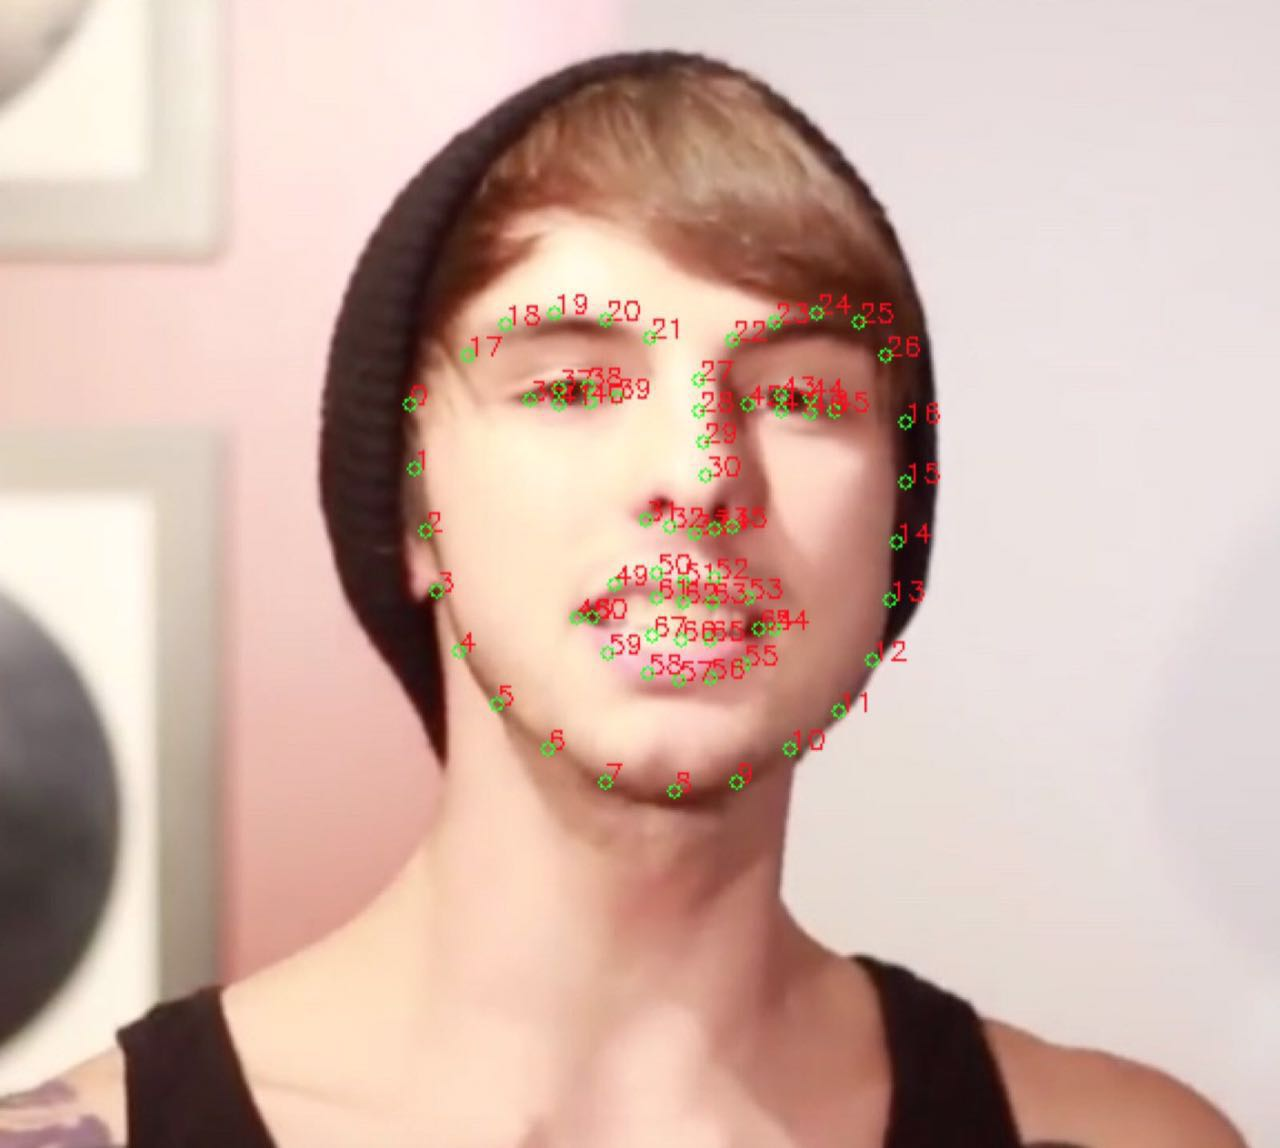
\includegraphics[width=0.5\linewidth]{5.jpg}
\caption{Detected face: cover artist M020}
\end{figure}

\item Estimate affine transform model
\item Estimate lip regions and Extract ROI
\begin{figure}
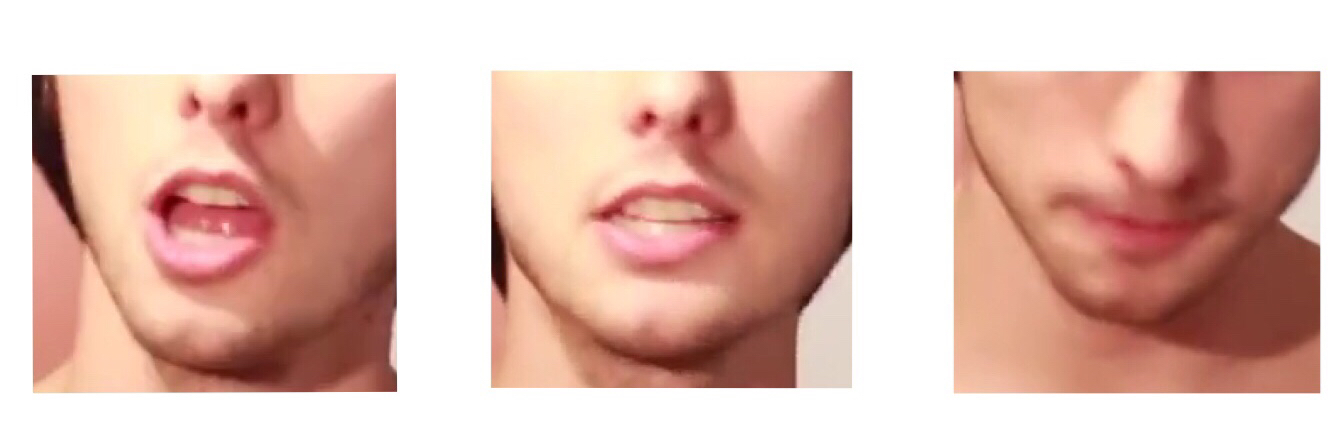
\includegraphics[width=0.8\linewidth]{frames.jpeg}
\caption{M020\_132\_01\_0101.00.027.mp4:\\
frame001 ,frame089 , frame152: 219x193}
\end{figure}
\item Convert to DCT
\begin{figure}
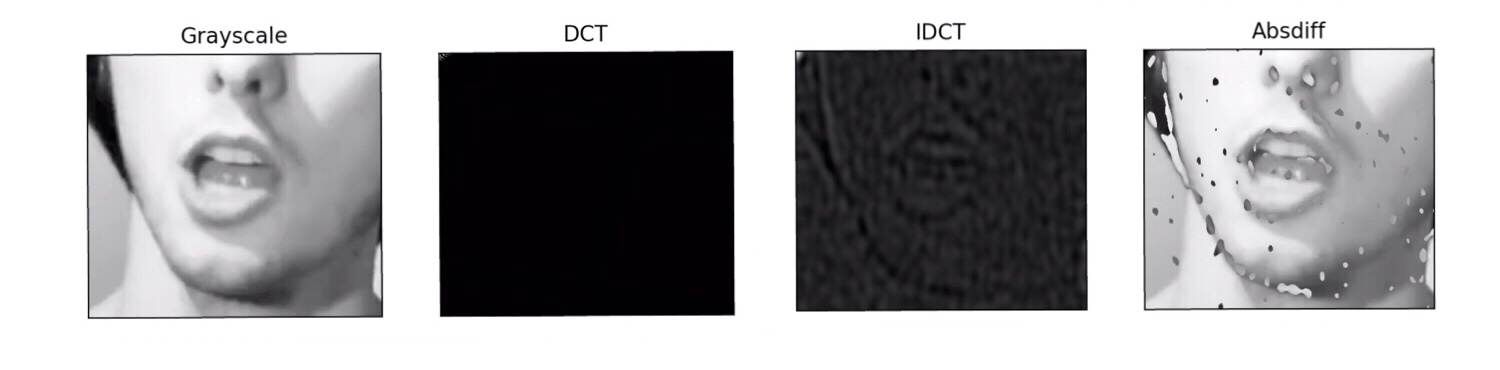
\includegraphics[width=0.9\linewidth]{dct.jpg}
\end{figure}
X=\bar{X}+P_{s}b_{s}




\end{enumerate}
\end{block}

\end{column} % End of column 2.1

\begin{column}{\onecolwid}\vspace{-.6in} % The second column within column 2 (column 2.2)

%----------------------------------------------------------------------------------------
%	Bad lip reading
%----------------------------------------------------------------------------------------

\begin{block}{Bad Lip reading}
\textbf{Bad Lip Reading}\cite{BLR} is a YouTube channel,work to recompose films, TV shows, songs, sports, and political news stories by overdubbing humorous vocal that matches the lip movements of targets. It shows that, even audio-only front end system is weak in robust noise, visual-only front end system is also not reliable. Here are two videos, one is the original MV called \textbf{'you\'re beautiful'} from famous singer \textbf{James Blunt}, and the other is from this channel.
 

\end{block}

%----------------------------------------------------------------------------------------

\end{column} % End of column 2.2

\end{columns} % End of the split of column 2 - any content after this will now take up 2 columns width

%----------------------------------------------------------------------------------------
%	
%----------------------------------------------------------------------------------------

\begin{alertblock}{System implementation in Kaldi}
\begin{figure}
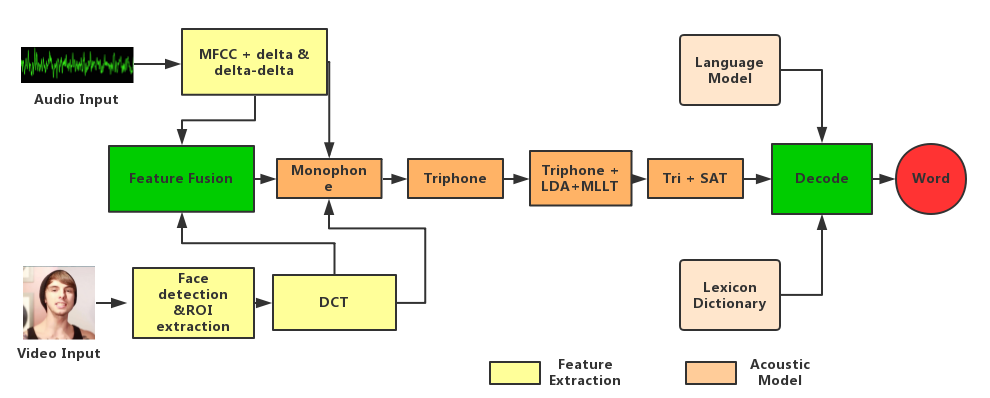
\includegraphics[width=1\linewidth]{dia.jpg}
\end{figure}
\end{alertblock} 



\end{column} % End of the second column

\begin{column}{\sepwid}\end{column} % Empty spacer column

\begin{column}{\onecolwid} % The third column

%----------------------------------------------------------------------------------------
%	CHALLENGE
%----------------------------------------------------------------------------------------

\begin{block}{Challenge}
\begin{itemize}
\item Too much Noise (Instrument Sound) in audio background
\item Too much useless sense for shotting instrument in videos
\item Multi-faces in one video
\item Artists do not frontally face to the camera 
\item Barriers like microphone or glasses shaded the lip and face
\item Adapt visual features into kaldi format and get fusion with audio features
\end{itemize}



\end{block}

%----------------------------------------------------------------------------------------
%	EXPERIMENTAL RESULTS
%----------------------------------------------------------------------------------------

\begin{block}{Experimental results}

\begin{table}
\vspace{2ex}
\begin{tabular}{l l}
\toprule
\textbf{System Front End    } & \textbf{   Average WER}\\
\midrule
Audio-only ASR    &    93.94\\
Visual-only ASR    &   98.49 \\

\bottomrule
\end{tabular}
\caption{Audio-only ASR system VS Visual-only ASR system}
\end{table}

\end{block}
%----------------------------------------------------------------------------------------
%	Conclusion
%----------------------------------------------------------------------------------------

\begin{block}{Conclusion}
The WER result of audio-only and Visual-only ASR systems are really bad. It may caused by the instrument background as noise and the limited size of our music corpus. Besides, as the videos showed in bad lip reading section, it makes a point that lip cues are ambiguous. We can not expect the visual-only system works well.
Therefore, it is necessary to develop a AV-ASR system in the future. However, the audio-visual feature integration is a vital problem for our feature level fusion's HMM-GMM model ASR system.


\end{block}

%----------------------------------------------------------------------------------------
%	REFERENCES
%----------------------------------------------------------------------------------------

\begin{block}{References}

\nocite{*} % Insert publications even if they are not cited in the poster
\small{\bibliographystyle{unsrt}
\bibliography{sample}\vspace{0.75in}}

\end{block}



\end{column} % End of the third column

\end{columns} % End of all the columns in the poster


\end{document}
